\section{Adopted Data}

The geometric data and the internal layout of the Exocet MM40 were taken from:
\url{http://sistemasdearmas.com.br/asv/exocet1historia.html}.

\begin{figure}[H]
\centering
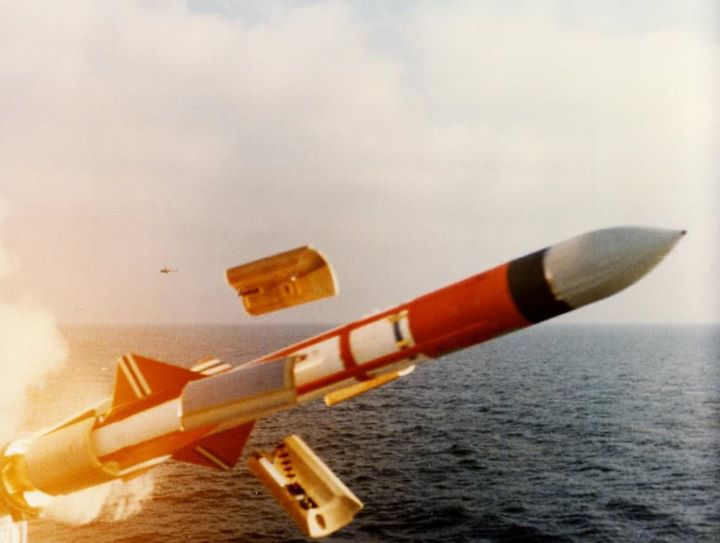
\includegraphics[width=0.72\textwidth]{images/exocetmm40.jpg}
\caption{External reference used to define the equivalent geometry.}
\end{figure}

\begin{table}[H]
\centering
\caption{Main adopted parameters.}
\begin{tabular}{lc}
\toprule
Parameter & Value \\
\midrule
Total length & 5.79 m \\
Diameter & 0.35 m \\
Wingspan & 1.13 m \\
Launch mass & 875 kg \\
DATCOM moment reference & 2.70 m \\
Mach range & 0.6 to 1.0 \\
Angle-of-attack range & -20 to 20 deg \\
Control deflection range & -20 to 20 deg \\
\bottomrule
\end{tabular}
\end{table}

\subsection*{Modeling assumptions}

The missile was treated as an equivalent Exocet-class configuration, not as an exact reverse-engineered model. The external dimensions came from the reference page, while the internal mass split was estimated from the subsystem figure and from the previous solid-propulsion sizing. The DATCOM model used an axisymmetric body with two fin sets and a fixed moment reference at \(X=2.70\) m. This point is close to, but not identical to, the estimated initial CG. The 6DOF simulation kept the course Simulink model and replaced only the missile data, CG/inertia data, launch condition, and aerodynamic matrix. The 6DOF run was used as an initial dynamic check of the generated coefficient bank, with emphasis on the alpha versus delta response.
